\documentclass[a4paper,14pt]{extarticle} \usepackage[utf8]{inputenc}
\usepackage[T1]{fontenc}
\usepackage[margin=2.5cm]{geometry}

% Fonte Caladea se existir, senão lmodern
\IfFileExists{caladea.sty}{
  \usepackage{caladea}
}{
  \usepackage{lmodern} }
\usepackage{ragged2e}
\usepackage{graphicx}
\usepackage[portuguese]{babel}
\usepackage{wrapfig}
\usepackage{hyperref}
\usepackage{fancyhdr}
\usepackage{xcolor}
\usepackage{rotating}
\usepackage{titlesec}
\usepackage{epigraph}
\usepackage{dirtytalk}
\usepackage{indentfirst} % Indenta o primeiro parágrafo após seções

% Ajuste do recuo de parágrafo
\setlength{\parindent}{1.5em}

% Adjust headheight to remove LaTeX warning
\setlength{\headheight}{17.54163pt}

% Centralizar títulos
\titleformat{\section}
  {\normalfont\centering\bfseries\Large}{}{1em}{}

\titleformat{\subsection}
  {\normalfont\centering\bfseries\large}{}{1em}{}

\titleformat{\subsubsection}
  {\normalfont\centering\bfseries}{}{1em}{}

% -------------- Símbolos de Versículo e Resposta --------------
% Definição do símbolo (a “barrinha” inclinada)
\makeatletter
\newcommand{\vers@resp@sym}{%
  \raisebox{0.2ex}{\rotatebox[origin=c]{-20}{$\m@th\rceil$}}%
}
% macro interna que sobrepõe a barrinha e a letra V ou R
\newcommand{\vers@resp}[2]{%
  {\ooalign{%
     \hidewidth\kern#1\vers@resp@sym\hidewidth\cr
     #2\cr
  }}%
}
% comandos públicos \versicle e \response
\DeclareRobustCommand{\versicle}{\vers@resp{-0.1em}{V}}
\DeclareRobustCommand{\response}{\vers@resp{0pt}{R}}
\makeatother
% ^------------- Símbolos de Versículo e Resposta -------------^

% Rodapé com imagem e página
\pagestyle{fancy}
% ---- Cabeçalho ------------
\fancyhf[C]{}
% ----- Rodapé --------------
\fancyfoot[C]{%
  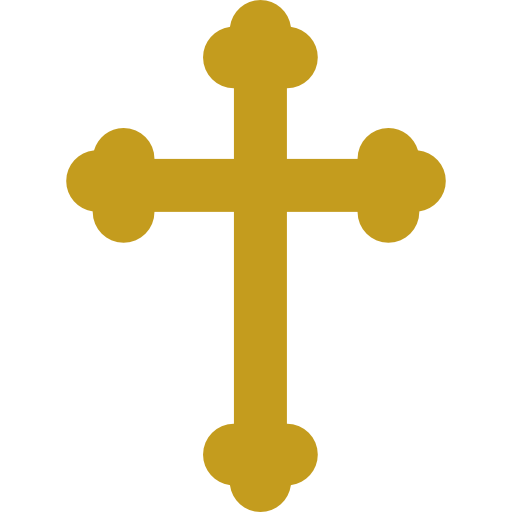
\includegraphics[scale=0.2]{assets/cross.png}\quad
  \textit{\textit{São Dimas, rogai por nós.}}\quad
  \thepage
}

\usepackage{pdfpages}
\begin{document}
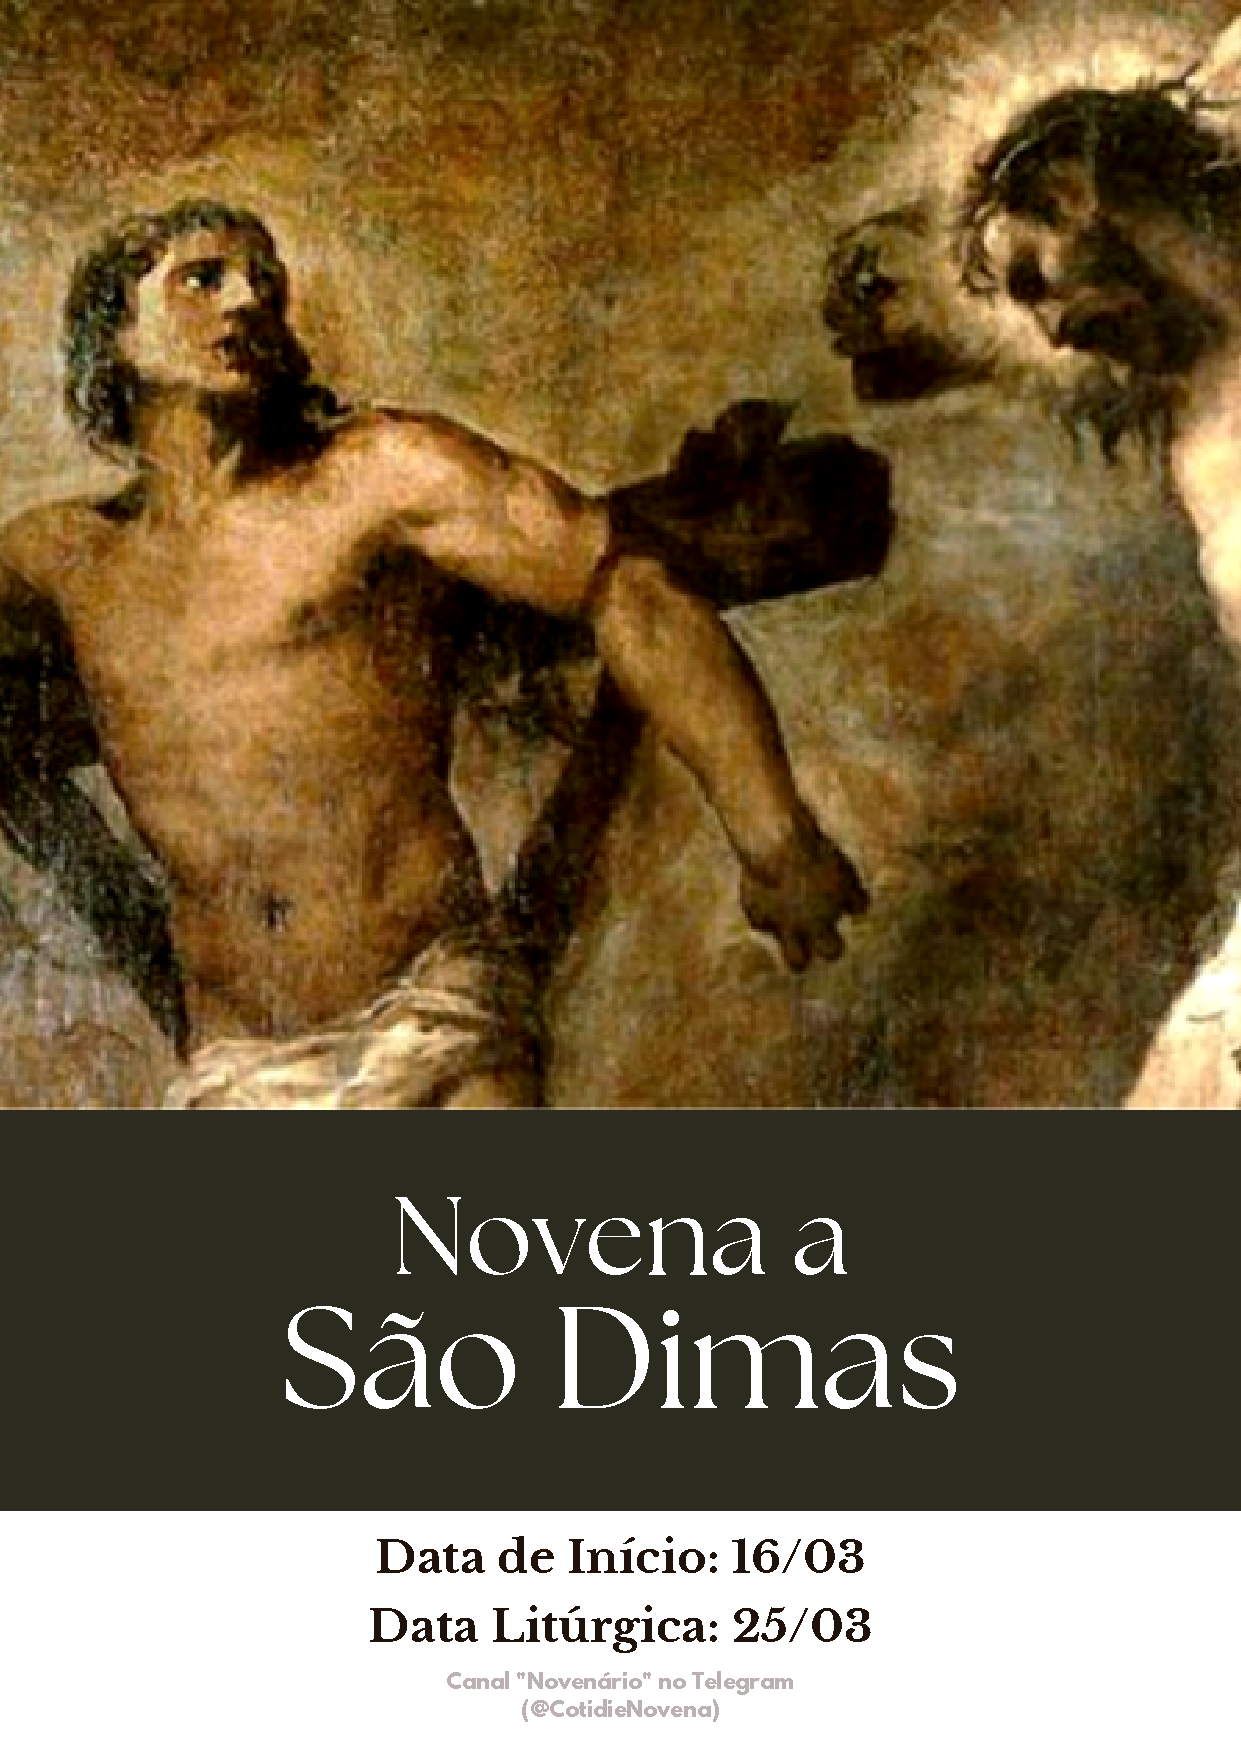
\includepdf[pages=1]{Capa São Dimas.pdf}

\begin{center}
	{\huge Novena de São Dimas}
\end{center}



\noindent\rule{\textwidth}{0.4pt}

\tableofcontents

\thispagestyle{empty}


% --- Origem ---
\newpage

\section{História}

Um dos episódios mais marcantes da crucificação de Jesus Cristo é o encontro com São Dimas, conhecido como “o bom ladrão”. Segundo a tradição, este homem conseguiu obter o Paraíso de Jesus no último momento, sendo condenado à morte ao lado do Messias. A história de São Dimas é repleta de simbolismos e lições de religiosidade.
\subsection{Quem foi Dimas?}

Uma das mais antigas lendas populares do cristianismo nos conta que o bom ladrão crucificado ao lado de Cristo se chamava Dimas. De acordo com a tradição, ele teria nascido em um covil de ladrões, filho do chefe do bando, e, ainda muito pequeno, teria contraído lepra.
image são dimas São Dimas esteve ao lado de Jesus na Crucificação

A lenda conta que o menino tornou-se um ladrão como seu pai. Quando adulto, acabou sendo capturado, conduzido a Jerusalém e condenado à morte por Pôncio Pilatos. Foi quando Dimas pôde ver Nosso Senhor carregando a cruz e sendo crucificado ao seu lado.

Ele se rendeu à graça de Deus e proclamou então aquele gesto de fé e de amor que ficou registrado para sempre no Evangelho; um gesto de fé que lhe rendeu a mais sublime promessa do próprio Filho de Deus: “Ainda hoje estarás comigo no Paraíso”.
\subsection{O Significado de São Dimas}

De fato, a história de São Dimas é cheia de simbolismos e ensinamentos. O bom ladrão representa o arrependimento e a redenção, demonstrando que, mesmo no último momento, é possível obter o perdão e a salvação.

Sua história é uma mensagem de esperança e misericórdia, inspirando a todos a buscarem a graça de Deus, independentemente de seus erros e pecados. Seu gesto de fé e amor é um exemplo do quanto a fé pode transformar vidas e garantir um lugar no Paraíso ao lado de Deus.
\subsection{Um Caso de Arrependimento e Esperança}

Sobre o episódio específico narrado no Evangelho, Santo Agostinho comentou:

\say{Eis aí, na Escritura, um caso de arrependimento no instante da morte, para que não nos desesperemos; porém, somente um, para que não presumamos.}

São Dimas, o bom ladrão, é um símbolo de que nunca é tarde para buscar a redenção e a salvação. Sua história nos ensina que, independentemente dos nossos erros, sempre podemos nos voltar para Deus e encontrar o perdão. A tradição o chama de padroeiro dos prisioneiros e moribundos, demonstrando que seu exemplo de arrependimento e fé continua inspirando e confortando milhares de pessoas ao redor do mundo.


% --- Orações Diárias ---
\newpage

\vfill

\section{Orações}
\subsection{Oração de Todos os Dias}\label{sub:inicial} % (fold)
São Dimas, a vossa confiança vos salvou na hora derradeira, e de grande pecador e criminoso que fostes, num instante, a misericórdia de Jesus vos transformou num grande Santo. Lembrai-vos de mim, pobre pecador como vós, e talvez maior do que vós, porque tenho abusado tanto da graça e ofendido tanto a Jesus Crucificado e morto por meu amor!
Pelas chagas do Divino Salvador no Calvário, pelas dores e as lágrimas de vossa Mãe, Maria Santíssima, alcançai-me a graça que ardentemente vos suplico; valei-me em minha aflição e em minhas necessidades temporais e espirituais! Assim seja.

\[\textbf{Pai Nosso, Ave-Maria e Gloria ao Pai.}\]

\vfill

\begin{center}
	\subsection*{Fontes:}
    Adaptado de: {\color{blue} \underline{\href{https://catolicoapp.com/santo/sao-dimas/}{Catolico App}}}
    e
    {\color{blue} \underline{\href{https://coracaofiel.com.br/novena/novena-de-sao-dimas/}{Coração Fiel}


  }

\end{center}


\end{document}
